A \cuda{} thread can be thought of as a lightweight thread, compared to a normal CPU thread.
It basically has access to the same resources but in a smaller scale.
As a kernel is executed in parallel by multiple threads, there must be a way to distinguish each thread from one another, so that they can perform different work.
Each thread is therefore given a \textit{thread index}, which can be accessed by each thread when executing a kernel.
It is syntactically done by accessing the struct \textit{threadIdx}, which contains the thread id in 3 dimension (x,y,z).
A simple example can be seen in \autoref{lst:threadIdx}.
\begin{lstlisting}[language=C,caption={Thread index example},label=lst:threadIdx]
__global__ void thread_idx_example(float* d_out, float* d_in){
	int idx = threadIdx.x;
	int idy = threadIdx.y;
	int idz = threadIdx.z; }
\end{lstlisting}
When a kernel is launched, the number of thread blocks (grid dimension) and the number of threads in a block (block dimension) must be specified.
The thread blocks are organized into a grid of blocks, in up to three dimensions (x,y,z).
In the same way, each block within the grid is comprised of multiple threads, also in up to three dimensions.
The thread hierarchy can be seen in \autoref{fig:grid-of-thread-blocks}, where the numbering is shown in "(x,y)" (z is zero in the example).
The grid dimension can be accessed by the struct \textit{gridDim}, The block id within the grid by \textit{blockIdx}, the block dimension by \textit{blockDim} and the thread id within a block by \textit{threadId}.
\begin{figure}[ht]
	\centering
	\fbox{
		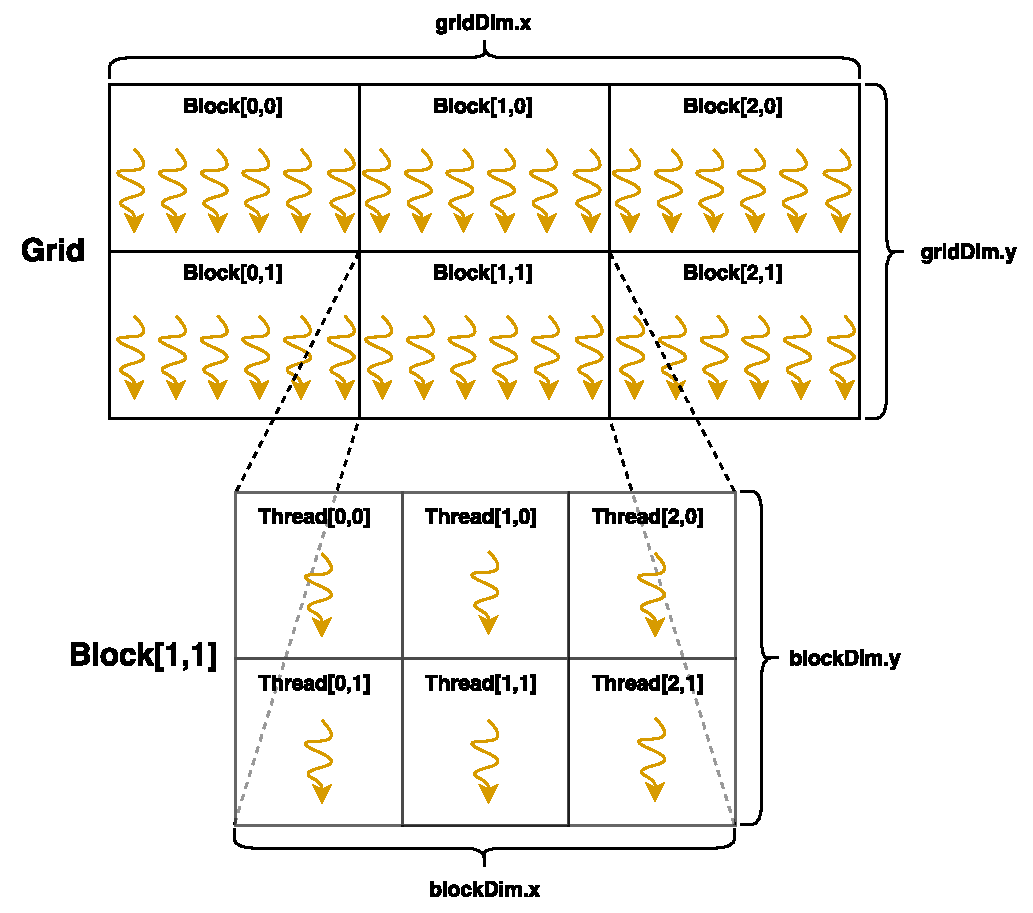
\includegraphics[width=0.6\textwidth]{figs/programming-model/grid-of-thread-blocks.pdf}
	}
	\caption{Grid of thread blocks}
	\label{fig:grid-of-thread-blocks}
\end{figure}
The maximum number of threads in a block is dependent on the specific device hardware, and on a lot of the current GPU's it can contain up to 1024 threads\cite{cuda:programmingguide}.
In \autoref{lst:thread-dim} is an example given of how to "create" a global thread id within the entire grid, so that each thread can perform independent work across thread blocks.
Another thing to notice is that to specify the size in three dimensions, the \textit{dim3} construct must be used.
\begin{lstlisting}[language=C,caption={Example of thread id usage in a grid of multiple thread blocks},label=lst:thread-dim]
__global__ void example(float * d_out, float * d_in){
	int myId = threadIdx.x + blockDim.x * blockIdx.x; }
int main(int argc, char ** argv) {
	dim3 blocks(x,y,z);
	dim3 threads(x,y,z);
	example<<<blocks, threads>>>(d_out, d_in); }
\end{lstlisting}
The number of blocks and threads to launch a kernel heavily depends on the specific application.
This is also valid in terms of the grid and block dimensions.
An example is that the dimensions can be chosen so that there is a natural mapping from a pixel in a picture, to each thread.
If the picture is black and white it would make sense to construct a 2D grid and if the picture contained RGB values, it would be preferable to construct a 3D grid.
So if the application contains multiple dimensions, it is possible to launch threads in multiple dimensions to ease the programming task.

